\documentclass[a4paper, 12pt]{article}
% math symbols
\usepackage{amssymb}
\usepackage{amsmath}
\usepackage{mathrsfs}
\usepackage{mathseries}


\usepackage[margin = 2cm]{geometry}

\tolerance = 1000
\emergencystretch = 0.74cm



\pagestyle{empty}

\setmathstyle{May 27}{School Algorithms, Combinatorics, and Complexity}{2021}

\begin{document}

    \begin{center}
    \textsc{A Few Words About the Proof Complexity}

    \textsc{Speaker: Dmitry Sokolov}
\end{center}

Proof system for a language $L \subseteq \{0, 1\}^*$ is a polynomial-time computable function
$\Pi\colon \{0, 1\}^* \times \{0, 1\}^* \rightarrow \{0, 1\}$ such that: 
\begin{enumerate}
	\item if $x \in L \Leftrightarrow$ there exists $y \in \{0, 1\}^*$ such that $\Pi(x, y) = 1$ (we say
        that $y$ is a proof of $x$);
	\item if $x \notin L \Leftrightarrow$ for all $y \in \{0, 1\}^*, \Pi(x, y) = 0$.
\end{enumerate}


The main task of proof complexity is to quantify the size of the smallest proof required to prove that
some given formula is unsatisfiable. Establishing superpolynomial lower bounds on the sizes in all proof
systems will imply that $\NP \neq \coNP$.

On the one hand in proof complexity, we can give the unconditional lower bounds on the length of proofs at
least in some proof systems (which in itself is valuable and amazing, unlike many other complexity
areas). On the other hand, we have lots of applications of these lower bounds: hard instances for
algorithms, lower bounds on the monotone complexity, etc. In this talk, we start with a brief description
of proof complexity and consider some applications.

\begin{center}
    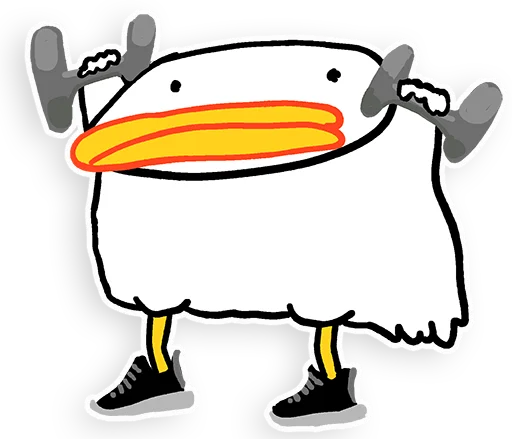
\includegraphics[scale = 0.1]{pics/utia-lift.png}
\end{center}

    \vspace{0.5cm}
    \begin{center}
    \textsc{Karchmer--Raz--Wigderson Conjecture}

    \textsc{Speaker: Ivan Mihajlin}
\end{center}


One of the major open problems in theoretic computer science is showing the existence of a problem that
could be solved in polynomial time but not by a logarithmic depth circuit (so-called $\P$ vs
$\NC_1$). One approach that has a lot of progress in the last several years is to prove Karchmer, Raz,
and Wigderson conjecture. It states that there is no better way to compute the composition of two
functions than applying them one by one. Lately, several interesting weaker versions of this conjecture
were proven using the language of communication complexity. We will discuss this conjecture, its relation
to circuit lower bounds, recent advances and hopes to prove it in the future.



    \vspace{1cm}
    \begin{center}
    \textsc{Data Structures Meet Circuits and Cryptography}

    \textsc{Speaker: Alexander Golovnev}
\end{center}



In this talk we will discuss the state of the art in the field of data structure lower bounds and
surprising connections between such lower bounds, circuit complexity, and cryptography. Proving such
limitations on data structures and circuits has been a fundamental research endeavor for several decades,
with connections to efficient parallel computation and the $\P$-vs-$\NP$ question. Despite much effort,
our best lower bounds in both fields have remained unchanged since the 1980s.

We show a surprising connection between both fields, offering an explanation for this lack of
progress. Specifically, we show that any improvement on the best known lower bound for a (linear) data
structure problem would imply new circuit lower bounds, and vice versa.

We continue this line of research by showing that data structure lower bounds for a specific class of
problems are equivalent to a certain kind of cryptography. We use this connection to construct surprising
(crypto-inspired) data structures for the $3\text{-}\langcplx{SUM}$ problem, refuting a data structure
variant of the $3\langcplx{SUM}$ conjecture due to Goldstein et al.
    
\end{document}